\ifx\pdfminorversion\undefined\else\pdfminorversion=4\fi
\documentclass[aspectratio=169,t]{beamer}
%\documentclass[aspectratio=169,t,handout]{beamer}

% English version FAU Logo
\usepackage[english]{babel}
% German version FAU Logo
%\usepackage[ngerman]{babel}

\usepackage[utf8]{inputenc}
\usepackage[T1]{fontenc}
\usepackage{amsmath,amssymb}
\usepackage{graphicx}
\usepackage{listings}
\usepackage{url}
\usepackage{enumitem}
\usepackage{hyperref}
\usepackage{fontawesome}
\usepackage{graphicx}
\usepackage{booktabs}
\usepackage{calc}
\usepackage{ifthen}
\usepackage{tikz}
\usepackage{tikz-cd}
\usepackage{pgfplots,pgfplotstable,pgf-pie}
\usepackage{filecontents}
\newcommand{\plots}{0.611201}
\newcommand{\plotm}{2.19882}
\pgfmathdeclarefunction{gauss}{2}{%
  \pgfmathparse{1/(#2*sqrt(2*pi))*exp(-((x-#1)^2)/(2*#2^2))}%
}

\tikzset{
    vertex/.style = {
        circle,
        fill            = black,
        outer sep = 2pt,
        inner sep = 1pt,
    }
}
\usetikzlibrary{matrix,mindmap}
\usetikzlibrary{arrows,decorations.pathmorphing,backgrounds,fit,positioning,shapes.symbols,chains,intersections,snakes}
\tikzset{level 1/.append style={sibling angle=50,level distance = 165mm}}
\tikzset{level 2/.append style={sibling angle=20,level distance = 45mm}}
\tikzset{every node/.append style={scale=1}}
% read in data file
\pgfplotstableread{data/iris.dat}\iris
% get number of data points
\pgfplotstablegetrowsof{\iris}
\pgfmathsetmacro\NumRows{\pgfplotsretval-1}

\usepgfplotslibrary{groupplots}
\pgfplotsset{height=4cm,width=8cm,compat=1.14}
\newcommand{\tikzmark}[1]{\tikz[remember picture] \node[coordinate] (#1) {#1};}
% Options:
%  - inst:      Institute
%                 med:      MedFak FAU theme
%                 nat:      NatFak FAU theme
%                 phil:     PhilFak FAU theme
%                 rw:       RWFak FAU theme
%                 rw-jura:  RWFak FB Jura FAU theme
%                 rw-wiso:  RWFak FB WISO FAU theme
%                 tf:       TechFak FAU theme
%  - image:     Cover image on title page
%  - plain:     Plain title page
%  - longtitle: Title page layout for long title
\usetheme[%
  image,%
  longtitle,%
  tf
]{fau}

% Enable semi-transparent animation preview
\setbeamercovered{transparent}


\lstset{%
  language=Python,
  tabsize=2,
  basicstyle=\tt,
  keywordstyle=\color{blue},
  commentstyle=\color{green!50!black},
  stringstyle=\color{red},
  numbers=left,
  numbersep=0.5em,
  xleftmargin=1em,
  numberstyle=\tt
}


% Title, authors, and date
\title[KDD]{Chapter II: Data}
\subtitle{Knowledge Discovery in Databases}
\author[L.~Melodia]{Luciano Melodia M.A.}
% English version
\institute[Department]{Evolutionary Data Management, Friedrich-Alexander University Erlangen-Nürnberg}
% German version
%\institute[Lehrstuhl]{Lehrstuhl, Friedrich-Alexander-Universit\"at Erlangen-N\"urnberg}
\date{Summer semester 2021}
% Set additional logo (overwrites FAU seal)
%\logo{\includegraphics[width=.15\textwidth]{themefau/art/xxx/xxx.pdf}}
\begin{filecontents}{data.dat}
  2 0.0629921259843
  3 0.0236220472441
  4 0.0314960629921
  5 0.125984251969
  6 0.0629921259843
  7 0.102362204724
  8 0.110236220472
  9 0.0551181102362
  10 0.0629921259843
  11 0.0314960629921
  12 0.0236220472441
  13 0.0314960629921
  14 0.0629921259843
  15 0.0551181102362
  16 0.0393700787402
  17 0.0472440944882
  18 0.00787401574803
  19 0.0393700787402
  24 0.00787401574803
  27 0.00787401574803
  33 0.00787401574803
\end{filecontents}

\begin{document}
\pgfplotstableread{
10.46365192956
90.22330318663
15.4712651178
80.87219994452
90.92824632322
80.69935247007
170.8222081627
140.3601041144
220.9047131581
80.05005282649
90.650706465
170.2352199894
70.76424153088
10.370245979
70.12513239519
20.64730407495
70.2072208982
14.7683650153
14.0063750733
19.324137585
20.40858604381
18.0368674939
80.02681240716
80.26418810694
120.1941169594
90.62080674537
30.24961728242
30.27316960403
170.9038479307
70.40481579419
10.814441695
80.40741573499
60.08031313304
130.1781459953
100.206134367
150.0864695726
90.03013313987
40.46906993699
90.27542593922
110.387166818
50.34088290758
70.35790199406
110.8693581818
100.8557924873
130.969617244
100.6354692297
30.03046442179
60.60358722529
120.2836888554
80.46665782108
130.9221860476
150.1323993544
70.16507829073
50.69317421704
150.4624253296
160.9138444234
60.44259653768
160.4478862876
30.46926929558
100.8862152053
100.4982459647
130.079580222
100.8219448481
120.1887774019
20.27608579327
40.21879129366
80.6626149873
30.05616084556
120.2628717929
30.07385860151
120.1834370192
70.86785100457
220.3039915506
70.6084726129
30.38040559575
40.77264935147
130.9493967532
140.1237678197
60.79956429934
80.7032357113
60.08645967617
90.19491098171
17.1651582777
40.7041931405
30.78091331321
50.20247821499
13.8921717364
60.09560236506
18.5811121283
10.3758110312
80.95955605147
12.4511725524
40.67834498484
11.0234433275
15.364443589
80.23928346825
60.30079928878
90.95330967273
12.5692010856
11.8362767596
}\datatable
\pgfplotstablesort{\sorted}{\datatable}
\pgfplotstablegetrowsof{\datatable}
\edef\numrows{\pgfplotsretval}

  % Title
  \maketitle

  {
    \setbeamertemplate{footline}[frame number]
    \begin{frame}{Chapter II: Getting to Know Your Data}
    This is our agenda for this lecture:
        \begin{itemize}
            \item \textbf{Data objects and attribute types.}
            \item Basic statistical descriptions of data.
            \item Data visualization.
            \item Measuring data similarity and dissimilarity.
            \item Summary.
        \end{itemize}
    \end{frame}
  }

  {
    \setbeamertemplate{footline}[frame number]
    \begin{frame}{Types of Data Sets}
      \begin{columns}
        \begin{column}{0.45\textwidth}
          \textbf{Records:}
          \begin{itemize}[noitemsep]
              \item Relational records.
              \item Data matrix, e.g. numerical matrix, crosstabs.
              \item Document data: text documents, \textbf{term-frequency vectors}. \tikzmark{n1}
              \item \textbf{Transaction data}. \tikzmark{n2}
          \end{itemize}
          \textbf{Graph and network:}
          \begin{itemize}[noitemsep]
              \item World wide web.
              \item Social of information networks.
              \item Molecular structures.
          \end{itemize}
        \end{column}
        \begin{column}{0.45\textwidth}  %%<--- here
        \begin{table}
         \begin{tabular}{|c|c|c|c|c|c|c|}
            \multicolumn{1}{c|}{} & \rotatebox[origin=c]{270}{team} & \rotatebox[origin=c]{270}{couch} & \rotatebox[origin=c]{270}{play} & \rotatebox[origin=c]{270}{ball} & \rotatebox[origin=c]{270}{score} & \rotatebox[origin=c]{270}{game} \\ \hline
            \tikzmark{t1} Document1 & 3 & 0 & 5 & 0 & 2 & 6 \\ \hline
            Document2 & 0 & 7 & 0 & 2 & 1 & 0 \\ \hline
            Document3 & 0 & 1 & 0 & 0 & 1 & 2 \\
            \hline
          \end{tabular}\\[0.5cm]
          \begin{tabular} { | c | l |}
          \hline
          \textbf{TID} & \textbf{Items} \\
          \hline
          \tikzmark{t2} 1 & Bread, Coke, Milk\\
          2 & Beer, Bread\\
          3 & Beer, Coke, Diapers, Milk\\
          4 & Beer, Bread, Diapers, Milk\\
          5 & Coke, Diapers, Milk \\
          \hline
          \end{tabular}
        \end{table}
        \begin{tikzpicture}[remember picture,overlay]
           \path[draw=blue,thick,->]<1-> ([yshift=1mm]n1) -- (t1);
           \path[draw=blue,thick,->]<1-> ([yshift=1mm]n2) -- (t2);
        \end{tikzpicture}
        \end{column}
      \end{columns}
    \end{frame}
  }

  {
    \setbeamertemplate{footline}[frame number]
    \begin{frame}{Types of Data Sets}
          \textbf{Ordered data:}
          \begin{itemize}[noitemsep]
              \item Video data: sequences of images.
              \item Temporal data: time series.
              \item Sequential data: transaction sequences.
              \item Genetic sequence data.
          \end{itemize}
          \textbf{Spatial, image and multimedia:}
          \begin{itemize}[noitemsep]
              \item Spatial data: maps.
              \item Image data.
              \item Video data.
          \end{itemize}
    \end{frame}
  }

  {
    \setbeamertemplate{footline}[frame number]
    \begin{frame}{Important Characteristics of Structured Data}
        \textbf{Dimensionality}:\\
        Curse of dimensionality (sparse high-dimensional data spaces).\\[0.2cm]
        % make the example with the volume of a cube

        \textbf{Sparsity}:\\
        Only presence counts.\\[0.2cm]

        \textbf{Resolution}:\\
        Patterns depend on the scale.\\[0.2cm]

        \textbf{Distribution}:\\
        Centrality and dispersion.
    \end{frame}
  }

  {
    \setbeamertemplate{footline}[frame number]
    \begin{frame}{Data Objects}
      \textbf{Data sets are made up of data objects}.\\
      \textbf{A data object represents an entity}.\\[0.2cm]

      Examples:
      \begin{itemize}
          \item Sales database: customers, store items, sales.
          \item Medical database: patients, treatments.
          \item University database: students, professors, courses.
      \end{itemize}

      They are also called:\\
      Sampels, examples, instances, data points, objects, tuples, \ldots\\[0.2cm]

      \textbf{Data objects are described by attributes}:
      \begin{itemize}
          \item Database rows $\rightarrow$ data objects.
          \item Columns $\rightarrow$ attributes.
      \end{itemize}
    \end{frame}
  }

  {
    \setbeamertemplate{footline}[frame number]
    \begin{frame}{Attributes}
    \textbf{Attribute}:\\
    Sometimes also in other context: field, dimension, feature, variable, \ldots\\[0.2cm]
    A data field encodes the property of an entity or feature of a data object.\\
    E.g. \texttt{customer\_ID}, \texttt{name}, \texttt{address}.\\[0.5cm]

    \textbf{Types}:
    \begin{itemize}
      \item Nominal.
      \item Binary.
      \item Ordinal.
      \item Numerical:
      \begin{itemize}
        \item Interval scaled.
        \item Ratio scaled.
      \end{itemize}
    \end{itemize}
    \end{frame}
  }

  {
    \setbeamertemplate{footline}[frame number]
    \begin{frame}{Attribute Types}
    \begin{itemize}
        \item \textbf{Nominal}:
        \begin{itemize}
            \item Categories, states, or "names of things".\\
                  E.g. \texttt{hair\_color} $= \{\text{auburn, black, blond, brown, grey, red, white}\}$.\\
                  Other examples: \texttt{marital\_status}, \texttt{occupation}, \texttt{ID}, \texttt{ZIP code}.
        \end{itemize}
        \item \textbf{Binary}:
            \begin{itemize}
                \item Nominal attribute with only two states ($0$ and $1$).
                \item \textbf{Symmetric binaries}: both outcomes equally important, such as \texttt{gender}.
                \item \textbf{Asymmetric binary}: outcomes not equally important. \\
                      E.g. medical test (positive vs. negative).\\
                      Convention: assign 1 to most important outcome (e.g. HIV positive).
            \end{itemize}
        \item \textbf{Ordinal}:
        \begin{itemize}
            \item Values have a meaningful order (ranking),\\
            but magnitude between successive values is not known.\\
            E.g. \texttt{size} $= \{\text{small, medium, large}\}$, grades, army rankings.
        \end{itemize}
        \end{itemize}
    \end{frame}
  }

  {
    \setbeamertemplate{footline}[frame number]
    \begin{frame}{Numerical Attribute Types}
    \begin{itemize}
        \item \textbf{Numerical: Quantity (integer- or real-valued)}.
        \item \textbf{Interval scaled}:
            \begin{itemize}
                \item Measured on a scale of \textbf{equally sized} units.
                \item Values have order.\\
                      E.g. temperature in $C$ or $F$, calender dates.
                \item No true zero-point.
            \end{itemize}
        \item \textbf{Ratio scaled}:
        \begin{itemize}
            \item Inherent \textbf{zero point}.
            \item We can speak of values as being an order of magnitude larger \\
            than the unit of measurement.\\
            E.g. $10 K$ is twice as high as $5 K$.\\
            E.g. temperature in Kelvin, length, counts, monetary quantities.
        \end{itemize}
        \end{itemize}
    \end{frame}
  }

  {
    \setbeamertemplate{footline}[frame number]
    \begin{frame}{Discrete vs. Continuous Attributes }
    \begin{itemize}
        \item \textbf{Discrete attribute}:
              \begin{itemize}
                  \item Has finite or countably infinite elements.\\
                        E.g. ZIP code, profession, or the set of words in a collection of documents.
                  \item Sometimes represented as integer variables.
                  \item Note: Binary attributes are a special case of discrete attributes.
              \end{itemize}
        \item \textbf{Continuous attribute}:
            \begin{itemize}
                \item Has real numbers as attribute values.\\
                      E.g. temperature, height, or weight.
                \item Practically, real values can only be measured and represented using a finite number of digits.
                \item Continuous attributes are typically represented as floating-point variables.
            \end{itemize}
        \end{itemize}
    \end{frame}
  }

  {
    \setbeamertemplate{footline}[frame number]
    \begin{frame}{Chapter II: Getting to Know Your Data}
        \begin{itemize}
            \item Data objects and attribute types.
            \item \textbf{Basic statistical descriptions of data.}
            \item Data visualization.
            \item Measuring data similarity and dissimilarity.
            \item Summary.
        \end{itemize}
    \end{frame}
  }

  {
    \setbeamertemplate{footline}[frame number]
    \begin{frame}{Basic Statistical Descriptions of Data}
    \textbf{Motivation}:
    \begin{itemize}
      \item To better understand the data: central tendency, variation and spread.
    \end{itemize}

    \textbf{Data dispersion characteristics}:
    \begin{itemize}
        \item Median, max, min, quantiles, outliers, variance etc.
    \end{itemize}

    \textbf{Numerical dimensions correspond to sorted intervals.}\\
    \begin{itemize}
      \item Data dispersion: analyzed with multiple granularities of precision.
      \item Boxplot or quantile analysis on sorted intervals
    \end{itemize}

  \textbf{Dispersion analysis on computed measures.}\\
    \begin{itemize}
        \item Folding measures into numerical dimensions.
        \item Boxplot or quantile analysis on the transformed cube.
    \end{itemize}
    \end{frame}
  }

  {
    \setbeamertemplate{footline}[frame number]
    \begin{frame}{Measuring the Central Tendency (I)}
    \begin{itemize}
      \item \textbf{Mean}:
      \begin{itemize}
          \item $N$ denotes the amount of samples within the data set.
          \item The \textbf{sample mean} is given by\\
                \begin{equation*}
                  \bar{x} = \frac{1}{N} \sum_{i=1}^{N} x_i.
                \end{equation*}
          \item While the \textbf{population mean} is defined by
                \begin{equation*}
                  \mu = \sum x \cdot p(x | \theta) \cdots.
                \end{equation*}
      \end{itemize}
    \end{itemize}
    \end{frame}
  }

  {
    \setbeamertemplate{footline}[frame number]
    \begin{frame}{Measuring the Central Tendency (II)}
      \begin{columns}
        \begin{column}{0.6\textwidth}
          \textbf{Median:}
          \begin{itemize}[noitemsep]
            \item The median $\tilde{x}$ minimizes the sum of absolute deviations for any $x$ of a sample $X$:
            \begin{align}
              \sum_{i=1}^{n} |\tilde{x}-x_i| \leq \sum_{i=1}^{n} |x-x_i|.
            \end{align}
            \begin{align}
              \tilde{x} = \begin{cases}
              x_{\frac{N}{2}} & \text{if $N$ mod $2 = 0$,} \\
              \frac{x_{\frac{N-1}{2}}+x_{\frac{N+1}{2}}}{2} & \text{if $N$ mod $2 \neq 0$.}
            \end{cases}
            \end{align}
          \end{itemize}
        \end{column}
        \begin{column}{0.3\textwidth}  %%<--- here
        \begin{table}
        \begin{tabular}{|c|c|}
          Age & Frequency \\ \hline
          $1-5$ & $200$ \\
          $6-15$ & $450$ \\
          $16-20$ & $300$ \\
          $21-50$ & $1500$ \\
          $51-80$ & $700$ \\
          $81-110$ & $44$
        \end{tabular}\\[0.5cm]
        \end{table}
        \end{column}
      \end{columns}
    \end{frame}
  }

  {
    \setbeamertemplate{footline}[frame number]
    \begin{frame}{Measuring the Central Tendency (III)}
      \begin{columns}
        \begin{column}{0.6\textwidth}
          \textbf{Median for interval grouped data:}
          \begin{itemize}[noitemsep]
            \item Let $n$ be the total amount of data points, $n_i$ the respective number of the $i$th group and $l_i$ or $u_i$ the lower or upper interval limit. We determine the group to which the median belongs and denote it as $m$th group. It is determined by
            \begin{align}
              \sum_{k=1}^{m-1}n_k < \frac{n}{2}, \; \text{but} \; \sum_{k=1}^{m} n_k \geq \frac{n}{2}.
            \end{align}
            \item If there is no information about the underlying distribution, we just assume that data is equally distributed and use linear interpolation to estimate the median:
            \begin{align}
              \tilde{x} = l_m + \frac{\frac{n}{2}-\sum_{k=1}^{m-1}n_k}{n_m} \cdot (u_m-l_m).
            \end{align}
          \end{itemize}
        \end{column}
        \begin{column}{0.3\textwidth}  %%<--- here
        \begin{table}
        \begin{tabular}{|c|c|}
          Age & Frequency \\ \hline
          $1-5$ & $200$ \\
          $6-15$ & $450$ \\
          $16-20$ & $300$ \\
          $21-50$ & $1500$ \\
          $51-80$ & $700$ \\
          $81-110$ & $44$
        \end{tabular}\\[0.5cm]
        \end{table}
        \end{column}
      \end{columns}
    \end{frame}
  }

  {
    \setbeamertemplate{footline}[frame number]
    \begin{frame}{Measuring the Central Tendency (IV)}
      \begin{columns}
        \begin{column}{0.6\textwidth}
          \textbf{Mode:}
          \begin{itemize}[noitemsep]
            \item Value that occurs most frequently within the data set.
            \item Can be unimodal, bimodal, trimodal etc.
            \item Empirical formula:
            \begin{align}
              \overline{x} - \text{mode} \approx 3(\overline{x}- \tilde{x}).
            \end{align}
          \end{itemize}
        \end{column}
        \begin{column}{0.3\textwidth}  %%<--- here
        \begin{table}
        \begin{tabular}{|c|c|}
          Age & Frequency \\ \hline
          $1-5$ & $200$ \\
          $6-15$ & $450$ \\
          $16-20$ & $300$ \\
          $21-50$ & $1500$ \\
          $51-80$ & $700$ \\
          $81-110$ & $44$
        \end{tabular}\\[0.5cm]
        \end{table}
        \end{column}
      \end{columns}
    \end{frame}
  }

  {
    \setbeamertemplate{footline}[frame number]
    \begin{frame}{Example of Mode, Median and Mean (I)}
      \centering
      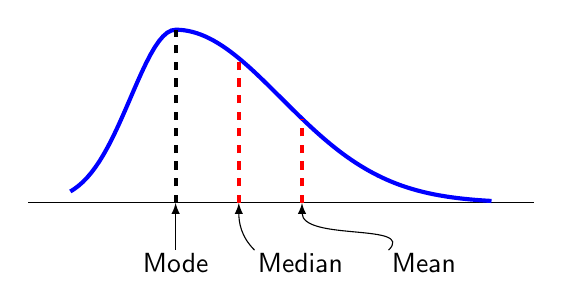
\begin{tikzpicture}[font=\sffamily,
      declare function={Gauss(\x,\y,\z,\u)=1/(\z*sqrt(2*pi))*exp(-((\x-\y+\u*(\x-\y)*sign(\x-\y))^2)/(2*\z^2));},
      every pin edge/.style={latex-,line width=1.5pt},
      every pin/.style={fill=yellow!50,rectangle,rounded corners=3pt,font=\small}]
      \begin{axis}[
          every axis plot post/.append style={
          mark=none,samples=101},
          clip=false,
          axis y line=none,
          axis x line*=bottom,
          ymin=0,
          xtick=\empty,]
          \addplot[line width=1.5pt,blue,domain=-1:3] {Gauss(x,0,0.6,-0.4)};
          \draw[line width=1.5pt,dashed, black] (0,0) -- (0,{Gauss(0,0,0.6,-0.4)});
          \draw[line width=1.5pt,dashed, red] (0.6,0) -- (0.6,{Gauss(0.6,0,0.6,-0.4)});
          \draw[line width=1.5pt,dashed, red] (1.2,0) -- (1.2,{Gauss(0.5,0,0.7,0.5)});
          \path (1.2,0) coordinate (ML) (0.6,0) coordinate (MR) (0,0) coordinate (MM);
      \end{axis}
      \draw[latex-] (ML) to[out=-90,in=45] ++ (1.1,-0.6) node[below right,inner
      sep=1pt]{Mean};
      \draw[latex-] (MR) to[out=-90,in=135] ++ (0.2,-0.6) node[below right,inner
      sep=1pt]{Median};
      \draw[latex-] (MM) --++ (0,-0.6) node[below,inner
      sep=1pt]{Mode};
      \end{tikzpicture}
      \begin{align}
        f(x \vert \mu, \sigma) = \frac{1}{\sqrt{2\pi\sigma^2}} \exp\left( - \frac{(x-\mu)^2}{2\sigma^2}\right).
      \end{align}
    \end{frame}
  }

  {
    \setbeamertemplate{footline}[frame number]
    \begin{frame}{Example of Mode, Median and Mean (II)}
    \textbf{Quartiles, outliers and boxplots:}
    \begin{itemize}
      \item \textbf{Quartiles:} {\color{blue}$\mathbf{Q}_1$} ($25^{\text{th}}$ percentile), {\color{blue}$\mathbf{Q}_3$} ($75^{\text{th}}$ percentile).
      \item \textbf{Inter quartile range:} {\color{blue}IQR} $=Q_3-Q_1$.
      \item Five number summary: min, $Q_1$, median, $Q_3$, max.
      \item \textbf{Boxplot}: ends of the box are the quartiles; \\ median is marked; add whiskers and plot outliers individually.
      \item \textbf{Outlier}: usually assigned to values higher/lower than $1.5 \cdot \text{IQR}$.
    \end{itemize}
    \textbf{Variance $\sigma^2$ and standard deviation $\sigma$}:
    \begin{itemize}
      \item Empirical sample variance: $\overline{\sigma^2} = \frac{1}{n-1} \sum_{i=1}^{n}(x_i-\overline{x})^2$
      \item Empirical population variance: $\sigma^2 = \frac{1}{N} \sum_{i=1}^{N} (x_i - \mu)^2$.
      \item Standard deviation is the square root $\sigma = \sqrt{\sigma^2}$.
    \end{itemize}
    \end{frame}
  }

  {
    \setbeamertemplate{footline}[frame number]
    \begin{frame}{Boxplot Analysis}
    \begin{center}
        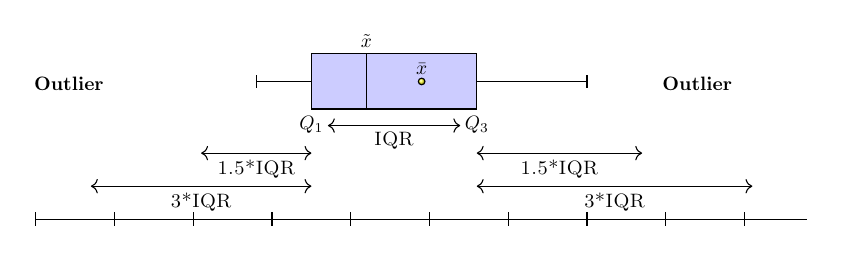
\begin{tikzpicture}[scale=0.7, transform shape]
            \filldraw[fill=blue!20] (2,0) rectangle (5,1);% draw the box
            \draw (3,0) -- (3,1) node[above]{$\tilde{x}$};% draw the median
            \draw (5,0.5) -- (7,0.5);% draw right whisker
            \draw (2,0.5) -- (1,0.5);% draw left whisker
            \draw (7,0.39) -- (7,0.61);% draw vertical tab
            \draw (1,0.39) -- (1,0.61);% draw vertical tab
            \node[below] at (2,0) {$Q_1$};% label the hinge
            \node[below] at (5,0) {$Q_3$};% label the hinge
            \filldraw[ball color=yellow!80,shading=ball] (4,0.5) circle
                (0.06cm) node[above]{$\bar{x}$};% the mean
            \draw[<->] (2.3, -0.3) -- (4.7, -0.3)
                node[pos=0.5,below]{$\textsc{IQR}$}; % mark the IQR fences
            \draw[<->] (2, -0.8) -- (0,-0.8)
                node[pos=0.5,below]{$\textsc{1.5*IQR}$}; % left inner fence
            \draw[<->] (2,-1.4) -- (-2, -1.4)
                node[pos=0.5,below]{$\textsc{3*IQR}$};% left outer fence
            \draw[<->] (5, -0.8) -- (8,-0.8)
                node[midway,below]{$\textsc{1.5*IQR}$}; % right inner fence
            \draw[<->] (5,-1.4) -- (10, -1.4)
                node[pos=0.5,below]{$\textsc{3*IQR}$};% right outer fence
            %
            \node[below] at (9,0.7) {$\textbf{Outlier}$}; % mild outlier on the right
            \node[below] at (-2.4,0.7) {$\textbf{Outlier}$}; % extreme outlier on the left
            % Axis
            \draw (-3,-2) -- (11,-2);
            % Note that the snaked line is drawn to 11.1 to force
            % TikZ to draw the final tick.
            \draw[snake=ticks,segment length=1cm] (-3,-2) -- (11.1,-2);
        \end{tikzpicture}
        \end{center}
          \textbf{Five number summary of a distribution:}\\
          Minimum, $Q_1$, median, $Q_3$, maximum.
          \\[0.2cm]
          \textbf{Boxplot}:
          \begin{itemize}
            \item Data is represented with a box.
            \item The ends of the box are at the first and third quartiles, i.e. the height of the box is IQR. \\
            The median is marked by a line within the box.
            \item Whiskers: two lines outside the box extended to minimum and maximum.
            \item Outliers: points beyond a specified outlier threshold, plotted individually.
          \end{itemize}
    \end{frame}
  }

  {
    \setbeamertemplate{footline}[frame number]
    \begin{frame}{Properties of Normal Distribution Curves}
    \begin{itemize}
        \item \textbf{The normal distribution:}
        \begin{itemize}
          \item From $\mu - \sigma$ to $\mu + \sigma$: contains about $68\%$ of the measurements.
          \begin{itemize}
              \item $\mu$: mean,
              \item $\sigma$: standard deviation.
          \end{itemize}
          \item From $\mu - 2 \sigma$ to $\mu + 2\sigma$: contains about $95\%$ of the surface under the curve.
          \item $\mu-3\sigma$ to $\mu + 3\sigma$: contains about $99.7\%$ of the surface under the curve.
        \end{itemize}
    \end{itemize}
    \vspace{0.2cm}
    \centering
    \begin{tikzpicture}
    \begin{axis}[
      no markers, domain=-3:3, samples=100,
      axis lines*=left, xlabel=$x$, ylabel=$y$,
      height=3.5cm, width = 5cm,
      xtick={-3,-2,-1,0,1,2,3}, ytick=\empty,
      enlargelimits=false, clip=false, axis on top,
      grid = major
      ]
      \addplot [fill=blue!20, draw=none, domain=-1:1] {gauss(0,1)} \closedcycle;
      \addplot [very thick,blue!50!black] {gauss(0,1)};
      \node[below] at (0,0.15) {$\approx 66 \%$};
    \end{axis}
    \end{tikzpicture}
    \hspace{0.2cm}
    \begin{tikzpicture}
    \begin{axis}[
      no markers, domain=-3:3, samples=100,
      axis lines*=left, xlabel=$x$, ylabel=$y$,
      height=3.5cm, width = 5cm,
      xtick={-3,-2,-1,0,1,2,3}, ytick=\empty,
      enlargelimits=false, clip=false, axis on top,
      grid = major
      ]
      \addplot [fill=blue!20, draw=none, domain=-2:2] {gauss(0,1)} \closedcycle;
      \addplot [very thick,blue!50!black] {gauss(0,1)};
      \node[below] at (0,0.15) {$\approx 95 \%$};
    \end{axis}
    \end{tikzpicture}
    \hspace{0.2cm}
    \begin{tikzpicture}
    \begin{axis}[
      no markers, domain=-3:3, samples=100,
      axis lines*=left, xlabel=$x$, ylabel=$y$,
      height=3.5cm, width = 5cm,
      xtick={-3,-2,-1,0,1,2,3}, ytick=\empty,
      enlargelimits=false, clip=false, axis on top,
      grid = major
      ]
      \addplot [fill=blue!20, draw=none, domain=-2.97:2.97] {gauss(0,1)} \closedcycle;
      \addplot [very thick,blue!50!black] {gauss(0,1)};
      \node[below] at (0,0.15) {$\approx 99.7 \%$};
    \end{axis}
    \end{tikzpicture}
    \hspace{0.2cm}
    \end{frame}
  }

{
  \setbeamertemplate{footline}[frame number]
  \begin{frame}{Visualization of Basic Statistical Descriptions}
  \begin{itemize}
    \item \textbf{Boxplot}: Visualization of five number summary.
    \item \textbf{Histogram}: $x$-axis are values, $y$-axis represent frequencies.
    \item \textbf{Quantile plot}: Each value $x_i$ is paired with some $q_i$ indicating that approximately $q_i \cdot 100 \%$ of data are $\leq x_i$.
    \item \textbf{Quantile-quantile (q-q) plot}: Graphs the quantiles of one univariate distribution against the corresponding quantiles of another.
    \item \textbf{Scatter plot}: Each pair of values is a pair of coordinates and plotted as points in the plane.
  \end{itemize}
  \end{frame}
}

{
  \setbeamertemplate{footline}[frame number]
  \begin{frame}{Histogram Analysis}
  \begin{itemize}
    \item \textbf{Histogram}: Visualization of tabulated frequencies, shown as bars.
    \item It shows what proportion of cases fall into each of several categories.
    \item Differs from a $\textbf{bar chart}$ in that it is the \emph{area} of the bar that denotes the value, not the height as in bar charts, a crucial distinction when the categories are not of uniform width.
    \item The categories are usually specified as non-overlapping intervals of some variable. The categories (bars) must be adjacent.
  \end{itemize}\vspace{0.2cm}
  \centering
  \begin{tikzpicture}
    \begin{axis}[
    yticklabel style={/pgf/number format/fixed},
    scaled y ticks = false,
    minor y tick num={1},
    xtick pos=left,
    legend cell align = left,
    legend style={draw=none},
    xlabel = {group size},
    ylabel = {ratio}
    ]
    \addplot[blue,ybar,fill, fill opacity=0.3, bar width = 0.8,] table {data.dat};
    \addplot[red, line width = 1,domain=1:40,samples=100] {1/(x*sqrt(2*pi)*\plots)*exp(-(ln(x)-\plotm)^2/(2*\plots^2))};
    \legend{empirical,lognormal fit}
    \end{axis}
  \end{tikzpicture}
  \end{frame}
}

{
  \setbeamertemplate{footline}[frame number]
  \begin{frame}{Histograms Often Tell More than Boxplots}
  The two histograms shown below may have the same boxplot representation, thus the same values for min, $Q_1$, median, $Q_3$ and for the max. But they have rather different underlying distributions.\\[1cm]
  \centering
  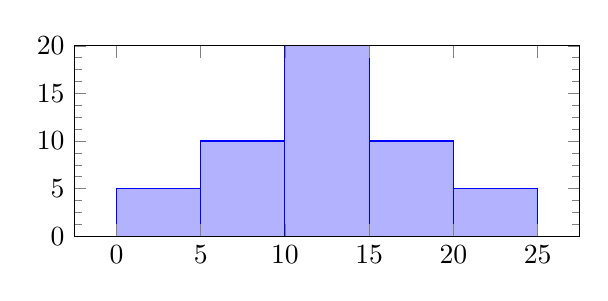
\begin{tikzpicture}
  \begin{axis}[
      ymin=0, ymax=20,
      minor y tick num = 3,
      area style,
      ]
  \addplot+[ybar interval,mark=no] plot coordinates {(0, 5) (5, 10) (10, 20) (15,10) (20,5) (25,5)};
  \end{axis}
  \end{tikzpicture}
  \hspace{0.5cm}
  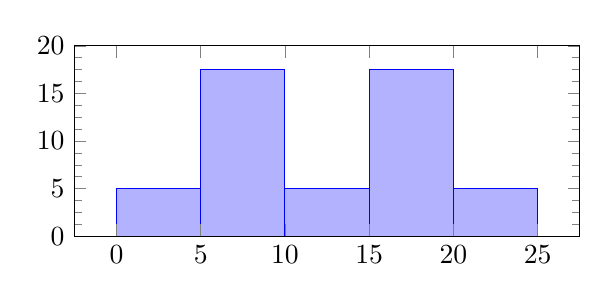
\begin{tikzpicture}
  \begin{axis}[
      ymin=0, ymax=20,
      minor y tick num = 3,
      area style,
      ]
  \addplot+[ybar interval,mark=no] plot coordinates {(0, 5) (5, 17.5) (10, 5) (15,17.5) (20,5) (25,5)};
  \end{axis}
  \end{tikzpicture}
  \end{frame}
}

  {
    \setbeamertemplate{footline}[frame number]
    \begin{frame}{Quantile Plot}
    \textbf{Displays all of the data.}\\
    A quantile plot allows the user to assess both the overall behaviour and unusual occurrences.\\[0.5cm]
    \textbf{Plots quantile information.}\\
    For some data point $x_i$, sorted in increasing order, $q_i$ indicates that approximately $q_i \cdot 100 \%$ of the data are below or equal to the value of $x_i$.\\[0.2cm]
    \centering
    \begin{tikzpicture}[
        declare function={norm(\x)=\x*\x/200;},
    ]
    \begin{axis}[
      ylabel={Unit price in \$},
      xlabel={q-value},
    ]
    \addplot[color=black, thick] table [x index=0, y index=0, x expr = \coordindex/100, y expr=norm(\coordindex)] {\sorted};
    \end{axis}
    \end{tikzpicture}
    \end{frame}
  }

  {
    \setbeamertemplate{footline}{
}    \begin{frame}{Quantile-quantile ($q-q$) Plot}
    \begin{itemize}
      \item Graphs the quantiles of one univariate distribution against the corresponding quantiles of another.
      \item View: Do these two distributions differ?\\
      Example shows unit price of items sold at Branch $1$ vs. branch $2$ for each quantile.  Unit prices of items sold at branch $1$ tend to be lower than those at branch $2$.
    \end{itemize}\vspace{0.5cm}
    \centering
    \begin{tikzpicture}[
        declare function={norm(\x)=2*\x;},
    ]
    \begin{axis}[
      ylabel={Branch 2 (unit price in \$)},
      xlabel={Branch 1 (unit price in \$)},
    ]
    \addplot [only marks, mark=*] table [x index=0, y index=0, y expr=norm(\coordindex)] {\sorted};
    \draw[black, thick] (0,0) -- (200,200);
    \end{axis}
    \end{tikzpicture}
    \end{frame}
  }

  {
    \setbeamertemplate{footline}[frame number]
    \begin{frame}{Scatter Plots}
    Provides a first look at \textbf{bivariate data} to see clusters of points, outliers or similar.\\
    Each pair of values is treated as a pair of coordinates and plotted as points in the plane.\\[0.5cm]
    \centering
    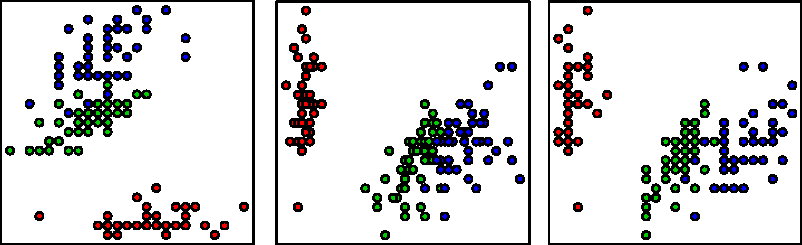
\includegraphics[height=3cm]{img/scatterplot.pdf}
    \end{frame}
  }

  {
    \setbeamertemplate{footline}[frame number]
    \begin{frame}{Data Profiling}
    \begin{itemize}
      \item \textbf{More from the database perspective.}
      \item \textbf{Derive metadata such as:}
      \begin{itemize}
        \item Data types and value patterns.
        \item Completeness and uniqueness of columns.
        \item Keys and foreign keys.
        \item Occasionally functional dependencies and association rules.
        \item Discovery of inclusion dependencies and conditional functional dependencies.
      \end{itemize}
      \item \textbf{Statistics:}
      \begin{itemize}
        \item Number of null values and distinct values in a column.
        \item Data types.
        \item Most frequent patterns of values.
      \end{itemize}
    \end{itemize}
    \end{frame}
  }

  {
    \setbeamertemplate{footline}[frame number]
    \begin{frame}{Chapter II: Getting to Know Your Data}
    \begin{itemize}
      \item Data objects and attribute types.
      \item Basic statistical descriptions of data.
      \item \textbf{Data visualization.}
      \item Measuring data similarity and dissimilarity.
      \item Summary.
    \end{itemize}
    \end{frame}
  }

  {
    \setbeamertemplate{footline}[frame number]
    \begin{frame}{Data Visualization}
    \textbf{Why visualize data?}
    \begin{itemize}
      \item \textbf{Gain insight} into an information space by mapping data into graphical primitives.
      \item \textbf{Provide qualitative overview} of large data sets.
      \item \textbf{Search} for patterns, trends, structure, irregularities, relationships among data.
      \item \textbf{Help find interesting regions and suitable parameters} for further quantitative analysis.
      \item \textbf{Provide a visual proof} of computer representations derived.
    \end{itemize}
    \textbf{Categorization of visualization methods:}
    \begin{itemize}
      \item Pixel-oriented.
      \item Geometric projection.
      \item Icon-based.
      \item Hierarchical.
      \item Visualizing complex data and relations.
    \end{itemize}
    \end{frame}
  }

  {
    \setbeamertemplate{footline}[frame number]
    \begin{frame}{Pixel Oriented Visualization Techniques}
    \begin{itemize}
      \item For a data set of $m$ dimensions create $m$ windows on the screen, one for each dimension.
      \item The values in dimension $m$ of a record are mapped to $m$ pixels at the corresponding \\ positions in the windows.
      \item The colors of the pixels reflect the corresponding values.
    \end{itemize}
    \vspace{0.5cm}
    \centering
    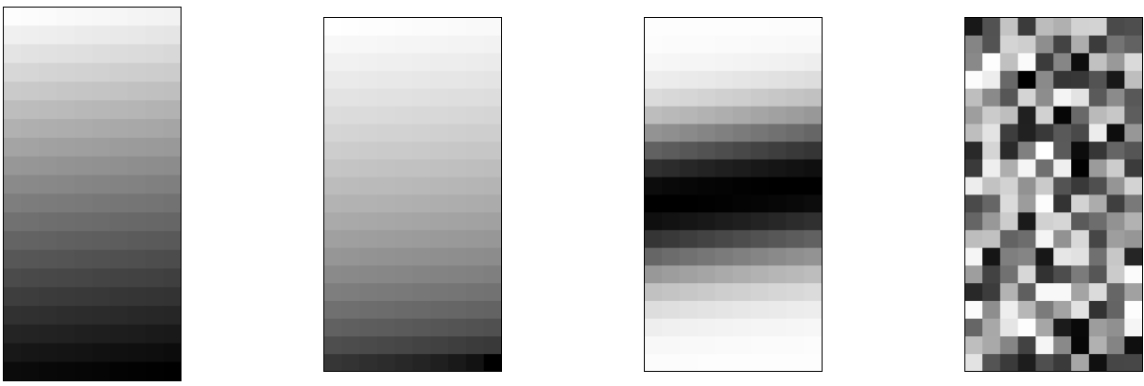
\includegraphics[width=9cm]{img/pixel.jpg}\\
    a) Income. \hspace{0.3cm} b) Credit limit. \hspace{0.2cm} c) Transaction volume. \hspace{0.2cm} (d) Age.
    \end{frame}
  }

  {
    \setbeamertemplate{footline}[frame number]
    \begin{frame}{Laying Out Pixels in a Spiderweb Diagram}
    To save space and show the connections among multiple dimensions, \\
    space filling is often done in a spiderweb diagram.\\
    \centering
    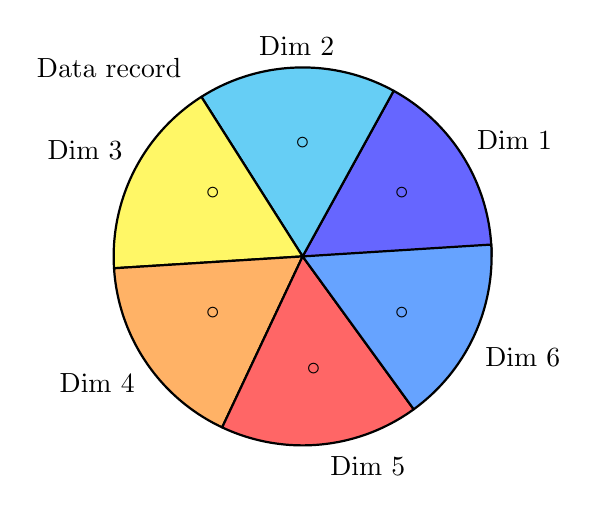
\begin{tikzpicture}[scale=0.8]
    \pie[hide number]{17/Dim 1, 17/Dim 2, 17/Dim 3, 17/Dim 4, 17/Dim 5, 16/Dim 6}
    \node at (1.5, 1) (a) {\tikzmark{t1} $\circ$};
    \node at (-1.5, 1) (b) {\tikzmark{t2} $\circ$};
    \node at (1.5, -0.9) (c) {\tikzmark{t3} $\circ$};
    \node at (-1.5, -0.9) (d) {\tikzmark{t4} $\circ$};
    \node at (0.1, -1.8) (e) {\tikzmark{t5} $\circ$};
    \node at (0, 1.8) (f) {\tikzmark{t6}$\circ$};
    \node at (-3, 3) (f) {Data record \tikzmark{n1}};
    \end{tikzpicture}
    \begin{tikzpicture}[remember picture,overlay]
      \path[draw=black,thick,-]<1-> (n1) -- (t1);
      \path[draw=black,thick,-]<1-> (n1) -- (t2);
      \path[draw=black,thick,-]<1-> (n1) -- (t3);
      \path[draw=black,thick,-]<1-> (n1) -- (t4);
      \path[draw=black,thick,-]<1-> (n1) -- (t5);
      \path[draw=black,thick,-]<1-> (n1) -- (t6);
    \end{tikzpicture}
    \end{frame}
  }

 {
    \setbeamertemplate{footline}[frame number]
    \begin{frame}{Laying Out Pixels in Circle Segments}
    To save space and show the connections among multiple dimensions, \\
    space filling is often done in a circle segment.\\
    \centering
    \newcommand{\D}{7} % number of dimensions (config option)
    \newcommand{\U}{7} % number of scale units (config option)

    \newdimen\R % maximal diagram radius (config option)
    \R=3.5cm
    \newdimen\L % radius to put dimension labels (config option)
    \L=4cm
    \newcommand{\A}{360/\D} % calculated angle between dimension axes

    \begin{tikzpicture}[scale=0.7]
      \path (0:0cm) coordinate (O); % define coordinate for origin

      % draw the spiderweb
      \foreach \X in {1,...,\D}{
        \draw (\X*\A:0) -- (\X*\A:\R);
      }

      \foreach \Y in {0,...,\U}{
        \foreach \X in {1,...,\D}{
          \path (\X*\A:\Y*\R/\U) coordinate (D\X-\Y);
          \fill (D\X-\Y) circle (1pt);
        }
        \draw [opacity=0.3] (0:\Y*\R/\U) \foreach \X in {1,...,\D}{
            -- (\X*\A:\Y*\R/\U)
        } -- cycle;
      }

      % define labels for each dimension axis (names config option)
      \path (1*\A:\L) node (L1) {Dim 1};
      \path (2*\A:\L) node (L2) {Dim 2};
      \path (3*\A:\L) node (L3) {Dim 3};
      \path (4*\A:\L) node (L4) {Dim 4};
      \path (5*\A:\L) node (L5) {Dim 5};
      \path (6*\A:\L) node (L6) {Dim 6};
      \path (7*\A:\L) node (L7) {Dim 7};

      % for each sample case draw a path around the web along concrete values
      % for the individual dimensions. Each node along the path is labeled
      % with an identifier using the following scheme:
      %
      %   D<d>-<v>, dimension <d> a number between 1 and \D (#dimensions) and
      %             value <v> a number between 0 and \U (#scale units)
      %
      % The paths will be drawn half-opaque, so that overlapping parts will be
      % rendered in a composite color.

      % Example Case 1 (red)
      %
      % D1 (Security): 0/7; D2 (Content Quality): 5/7; D3 (Performance): 0/7;
      % D4 (Stability): 6/7; D5 (Usability): 0/7; D6 (Generality): 5/7;
      % D7 (Popularity): 0/7
      \draw [color=red,line width=1.5pt,opacity=0.5]
        (D1-0) --
        (D2-5) --
        (D3-0) --
        (D4-6) --
        (D5-0) --
        (D6-5) --
        (D7-0) -- cycle;

      % Example Case 2 (green)
      %
      % D1 (Security): 2/7; D2 (Content Quality): 2/7; D3 (Performance): 5/7;
      % D4 (Stability): 1/7; D5 (Usability): 4/7; D6 (Generality): 1/7;
      % D7 (Popularity): 7/7
      \draw [color=green,line width=1.5pt,opacity=0.5]
        (D1-2) --
        (D2-2) --
        (D3-5) --
        (D4-1) --
        (D5-4) --
        (D6-1) --
        (D7-7) -- cycle;

      % Example Case 3 (blue)
      %
      % D1 (Security): 1/7; D2 (Content Quality): 7/7; D3 (Performance): 4/7;
      % D4 (Stability): 4/7; D5 (Usability): 3/7; D6 (Generality): 5/7;
      % D7 (Popularity): 2/7
      \draw [color=blue,line width=1.5pt,opacity=0.5]
        (D1-1) --
        (D2-7) --
        (D3-4) --
        (D4-4) --
        (D5-3) --
        (D6-5) --
        (D7-2) -- cycle;

    \end{tikzpicture}
    \end{frame}
  }

  {
    \setbeamertemplate{footline}[frame number]
    \begin{frame}{Geometric Projection Visualization Techniques}
    \begin{itemize}
      \item Visualization of geometric transformations and projections of data.
      \item \textbf{Methods}:
      \begin{itemize}
          \item Scatter plot and scatter plot matrices.
          \item Landscapes.
          \item Projection pursuit technique: \emph{Help users find meaningful projections of multidimensional data.}
          \item Prosection views.
          \item Hyperslice.
          \item Parallel coordinates.
      \end{itemize}
    \end{itemize}
    \end{frame}
  }

  {
    \setbeamertemplate{footline}[frame number]
    \begin{frame}{Scatter Plot Matrices}
    \centering
    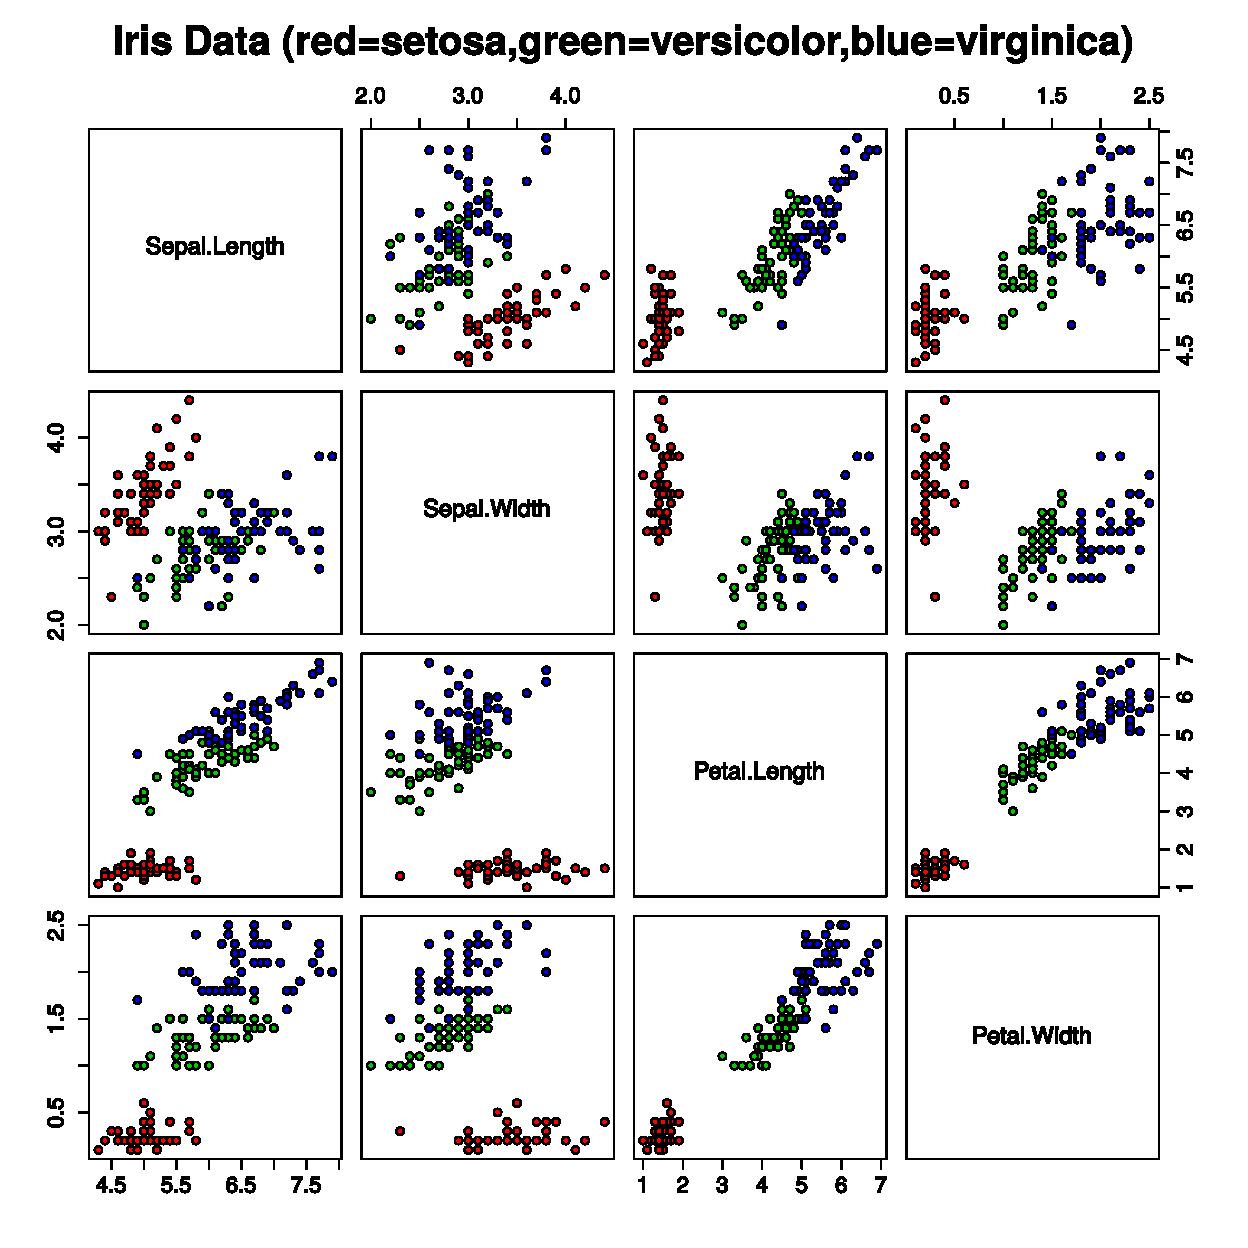
\includegraphics[height=6.5cm]{img/scatterplot_matrix.pdf}
    \end{frame}
  }

  {
    \setbeamertemplate{footline}[frame number]
    \begin{frame}{Parallel Coordinate Plot}
    \centering
    \vspace{0.5cm}
    \begin{tikzpicture}
    \begin{groupplot}[
      group style={
        group name=iris,
        group size=4 by 1,
        horizontal sep=2cm
      },
      axis y line=left,
      hide x axis,
      width=2cm,
      height=6cm,
      xmin=0,
      xmax=0.5,
      enlarge y limits,
      every axis plot/.append style={opacity=0}
    ]

    \nextgroupplot

    \pgfplotsinvokeforeach{0,...,\NumRows} % loop over all rows in table
    {
      % get value in sw column
      \pgfplotstablegetelem{####1}{sw}\of{\iris}%
       % add a coordinate at x=0 and that y-value
      \edef\temp{\noexpand\addplot coordinates {(0,\pgfplotsretval)} coordinate (sl####1);}
      \temp
    }

    \nextgroupplot

    \pgfplotsinvokeforeach{0,...,\NumRows}
    {
      \pgfplotstablegetelem{####1}{sl}\of{\iris}%
      \edef\temp{\noexpand\addplot coordinates {(0,\pgfplotsretval)} coordinate (sw####1);}
      \temp
    }

    \nextgroupplot

    \pgfplotsinvokeforeach{0,...,\NumRows}
    {
      \pgfplotstablegetelem{####1}{pw}\of{\iris}%
      \edef\temp{\noexpand\addplot coordinates {(0,\pgfplotsretval)} coordinate (pl####1);}
      \temp
    }

    \nextgroupplot

    \pgfplotsinvokeforeach{0,...,\NumRows}
    {
      \pgfplotstablegetelem{####1}{pl}\of{\iris}%
      \edef\temp{\noexpand\addplot coordinates {(0,\pgfplotsretval)} coordinate (pw####1);}
      \temp
    }

    \end{groupplot}

    % add labels below
    \foreach \i/\txt in {1/SW,2/SL,3/PW,4/PL}
      \node [below] at (iris c\i r1.south west) {\txt};


    % draw the lines
    % this dataset has three groups of fifty rows each, hence the start/stop values
    \foreach[
     evaluate=\j as \START using int(\j*50),
     evaluate=\j as \STOP using int((\j+1)*50-1),
      ] \j/\clr in {0/blue,1/red,2/green}
    {
    \foreach \i in {\START,...,\STOP}
       \draw [color=\clr,opacity=0.5] (sl\i) -- (sw\i) -- (pl\i) -- (pw\i);
    }

    \end{tikzpicture}
    \end{frame}
  }

  {
    \setbeamertemplate{footline}[frame number]
    \begin{frame}{Icon Based Visualization}
    \centering
    \begin{itemize}
      \item \textbf{Visualization of the data values as features of icons.}
      \item \textbf{Typical visualization methods:}
      \begin{itemize}
        \item Chernoff faces.
        \item Stick figures.
      \end{itemize}
      \item \textbf{General techniques:}
      \begin{itemize}
        \item Shape coding: \emph{Use shape to represent certain information encoding.}
        \item Color icons: \emph{Use color icons to encode more information.}
        \item Tile bars: \emph{Use small icons to represent the relevant feature vectors in document retrieval.}
      \end{itemize}
    \end{itemize}
    \end{frame}
  }

  {
    \setbeamertemplate{footline}[frame number]
    \begin{frame}{Chernoff Faces}
    \textbf{A way to display variables on a two-dimensional surface:}\\
    E.g. let $x$ be eyebrow slant, $y$ be eye size, $z$ be nose length etc.\\
    The figure shows faces produced using $10$ characteristics (head eccentricity, eye size, eye spacing, eye eccentricity, pupil size, eyebrow slant, nose size, mouth shape, mouth size, and mouth opening). Each assigned one of $10$ possible values, generated using \href{https://www.wolfram.com/mathematica/}{Mathematica} (S. Dickson).\\[0.5cm]
    \centering
    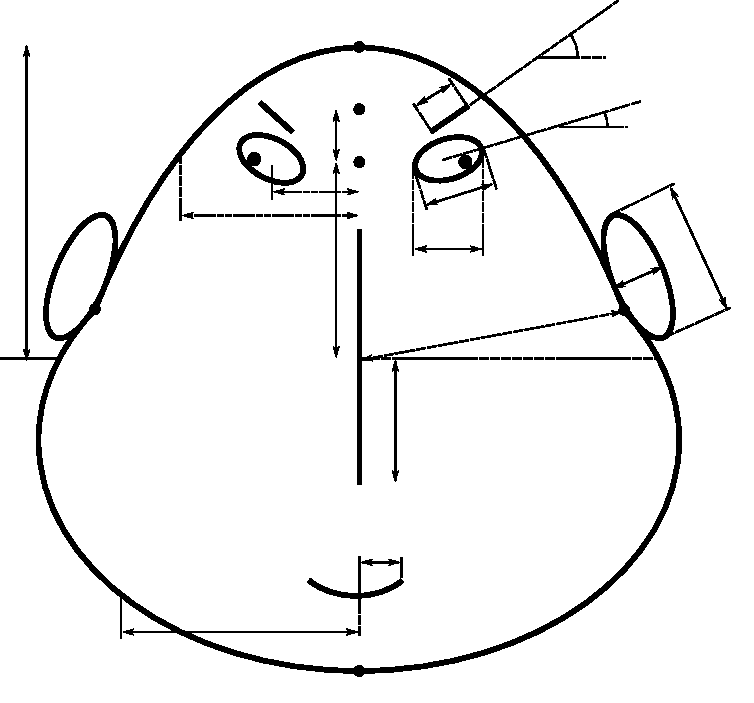
\includegraphics[width=4cm]{img/chernoff_faces_construction.pdf}
    \end{frame}
  }

  {
    \setbeamertemplate{footline}[frame number]
    \begin{frame}{Stick Figure}
    A census data figure showing age, income, gender, education etc. \\
    A $5$-piece stick figure ($1$ body and $4$ limbs w. different angle/length).\\[0.1cm]
    \centering
    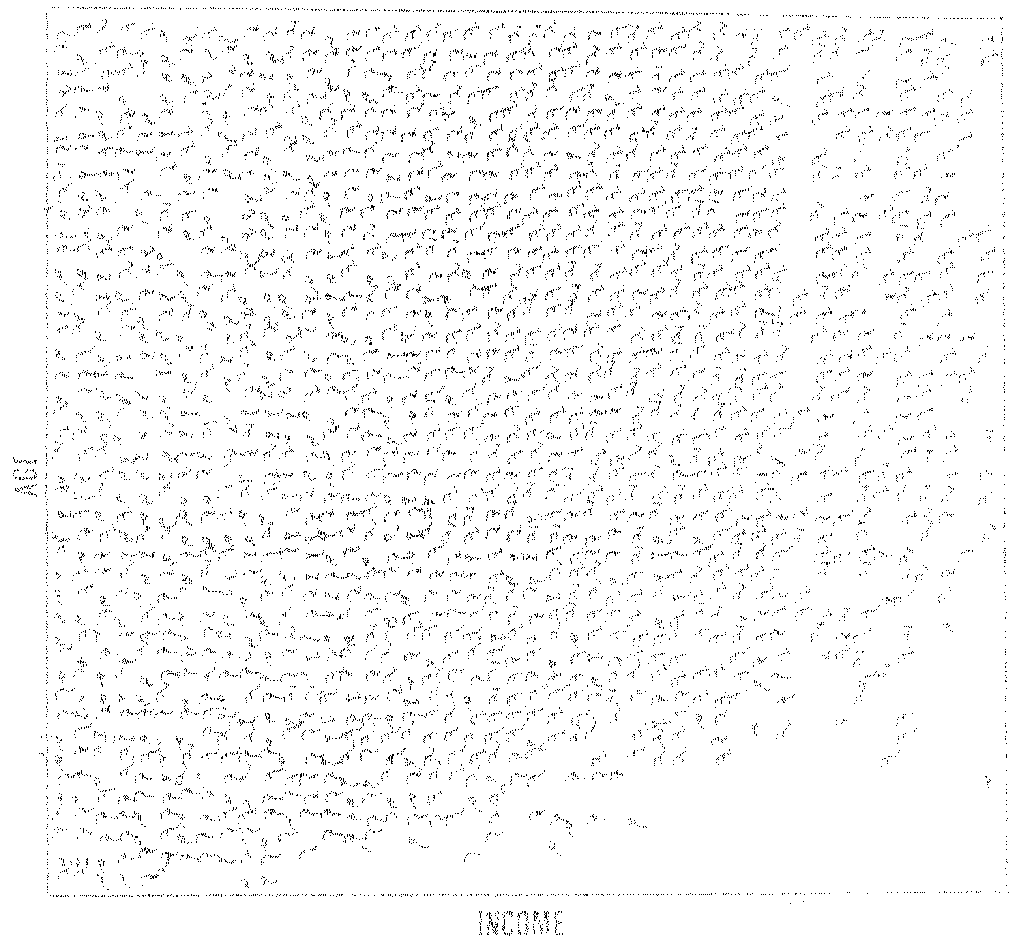
\includegraphics[width=8cm, height=5.2cm]{img/stick_figure.png}\\
    \tiny{Used by permission of G. Grinstein, University of Massachusettes at Lowell.}
    \end{frame}
  }

  {
    \setbeamertemplate{footline}[frame number]
    \begin{frame}{Hierarchical Visualization Techniques}
    \centering
    \begin{itemize}
      \item \textbf{Visualization of the data using a hierarchical partitioning into subspaces.}
      \item \textbf{Methods:}
      \begin{itemize}
        \item Worlds within worlds.
        \item Tree maps.
        \item Cone trees.
        \item Info cube.
      \end{itemize}
    \end{itemize}
    \end{frame}
  }

  {
    \setbeamertemplate{footline}[frame number]
    \begin{frame}{Worlds Within World}
    \begin{itemize}
      \item Assign the function and two most important parameters to innermost world.
      \item Fix all other parameters at constant values -- draw other (1,2 or 3) dimensional worlds choosing these as the axes.
    \end{itemize}
    \centering
    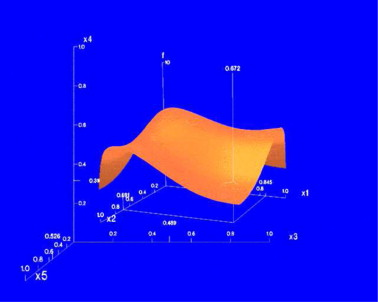
\includegraphics[width=8cm,height=5.2cm]{img/www.jpg}
    \end{frame}
  }

  {
    \setbeamertemplate{footline}[frame number]
    \begin{frame}{Tree Maps}
    \centering
    \begin{itemize}
      \item \textbf{Screen filling method:}
      \begin{itemize}
        \item Uses a hierarchical partitioning of the screen into regions depending on the attribute values.
        \item $x$ and $y$-coordinates of the screen partitioned alternately according to the attribute values.
      \end{itemize}
    \end{itemize}
    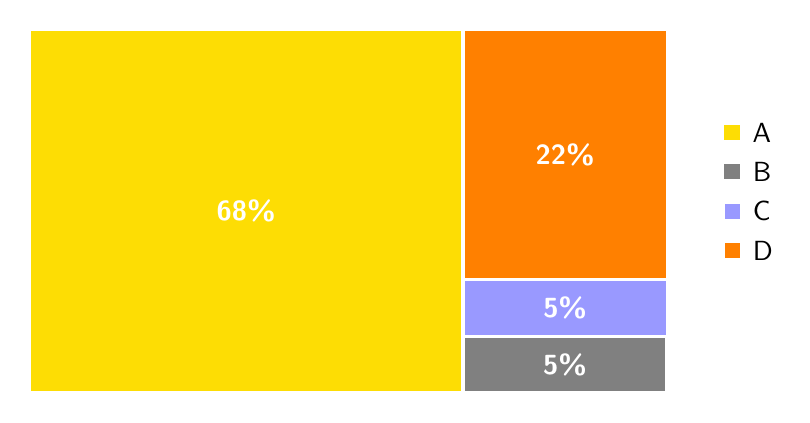
\begin{tikzpicture}[xscale = 1.35, yscale = 0.77,
     font=\sffamily,
    mystyle/.style={draw=white, very thick, text=white, font=\sffamily\bfseries},
    ]
    \pie[square,
    style={mystyle},
    color={yellow!80!orange, gray, blue!40, orange},
    text=legend,
    ]{68/A, 5/B, 5/C, 22/D}
    \end{tikzpicture}
    \end{frame}
  }

  {
    \setbeamertemplate{footline}[frame number]
    \begin{frame}{Tree Map of a File System}
    \centering
    \vspace{0.5cm}
    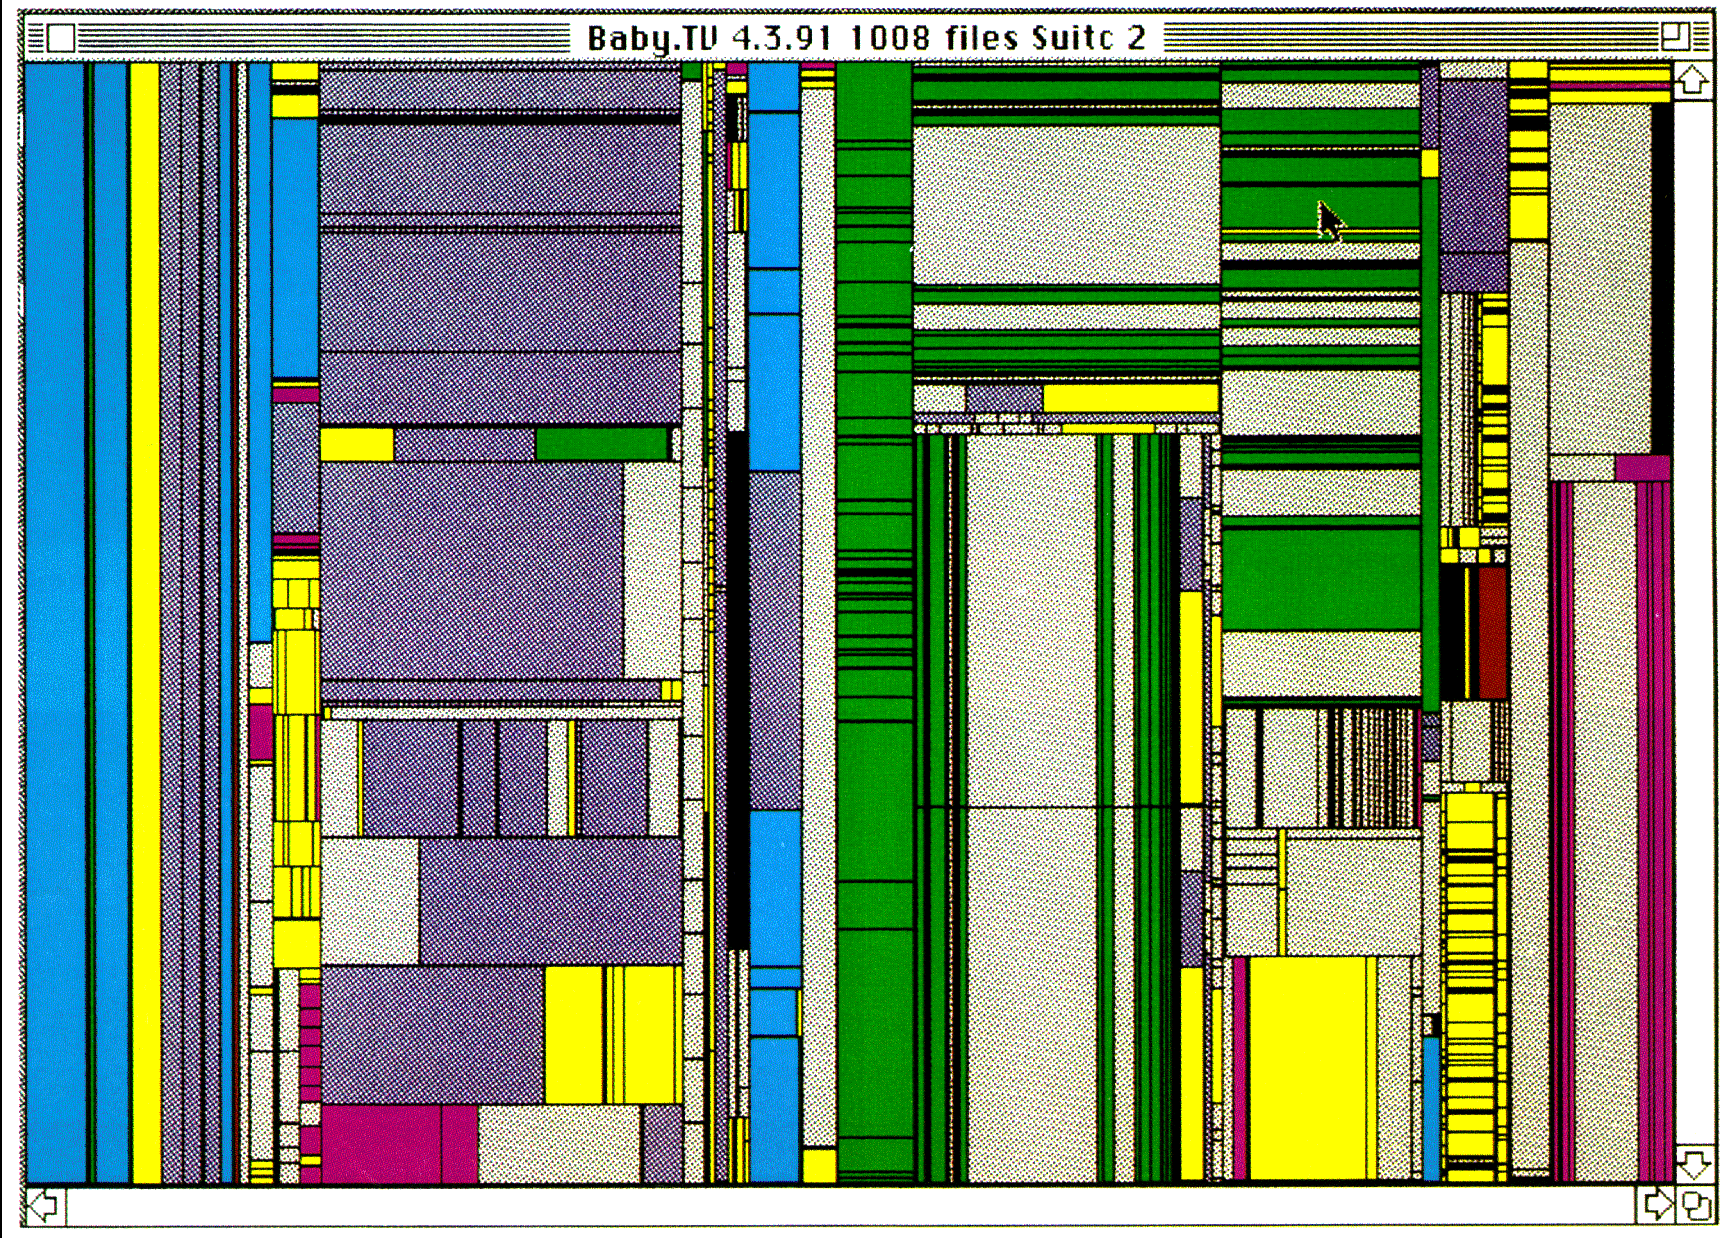
\includegraphics[width=9cm, height=6cm]{img/treemap_filesystem.png}
    \end{frame}
  }

  {
    \setbeamertemplate{footline}[frame number]
    \begin{frame}{Info Cubes}
    \begin{itemize}
      \item $3$D visualization technique:
      \begin{itemize}
        \item Hierarchical information is displayed as nested semi-transparent cubes.
        \item The outermost cubes correspond to the top level data, while the subnodes or the lower level data are represented as smaller cubes inside the outermost cubes, and so on.
      \end{itemize}
    \end{itemize}
    \vspace{0.2cm}
    \centering
    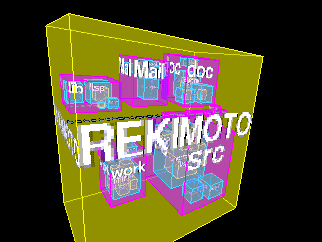
\includegraphics[width=4cm,height=4cm]{img/infocube.png}
    \end{frame}
  }

  {
    \setbeamertemplate{footline}[frame number]
    \begin{frame}{Three Dimensional Cone Trees}
    \centering
    \begin{itemize}
      \item $3$D cone-tree visualization technique:\\
            works well for up to approx. a thousand nodes.
      \item Build a $2$D circle tree that arranges its nodes in concentric circles centered on the root node.
      \item Overlaps can't be avoided projecting onto $2$D.
      \item G. Robertson, J. Mackinlay, S. Card. "Cone Trees: Animated 3D Visualizations of Hierarchical Information", ACM SIGCHI'91.
    \end{itemize}
    \vspace{0.2cm}
    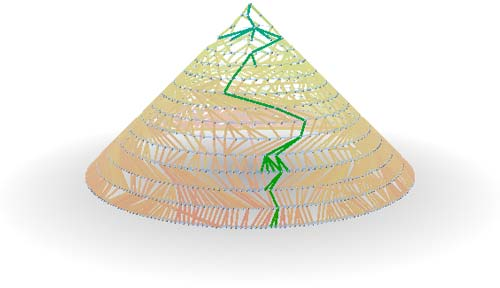
\includegraphics[width=3cm,height=3cm]{img/threedcone_one.jpg}\hspace{1cm}
    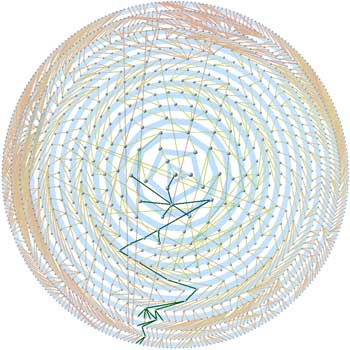
\includegraphics[width=3cm,height=3cm]{img/threedcone_two.jpg}\\
    \tiny{Acknowledgement: \href{ttp://nadeausoftware.com/articles/visualization}{http://nadeausoftware.com/articles/visualization}.}
    \end{frame}
  }

  {
    \setbeamertemplate{footline}[frame number]
    \begin{frame}{Visualizing Complex Data and Relations}
    \centering
    \begin{itemize}
      \item \textbf{Visualizing non-numerical data: text and social networks.}
      \item \textbf{Tag cloud: visualizing user-generated tags.}
      \begin{itemize}
        \item The importance of tag is represented by font size/color.
        \item Besides text data, there are also methods to visualize relationships, \\ such as visualizing social networks.
      \end{itemize}
    \end{itemize}
    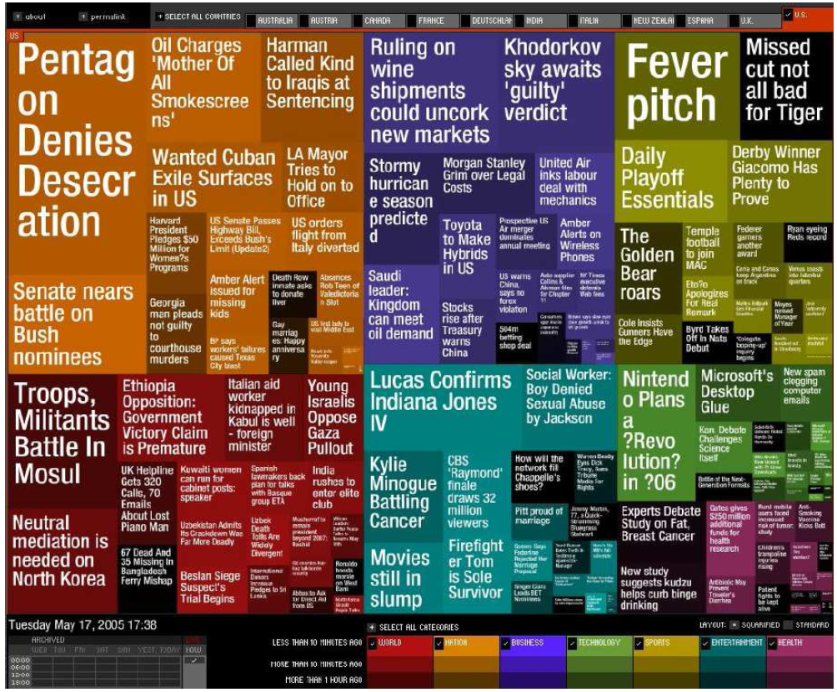
\includegraphics[width=7cm,height=4cm]{img/google_news.png}
    \end{frame}
  }

  {
    \setbeamertemplate{footline}[frame number]
    \begin{frame}{Chapter 2: Getting to Know Your Data}
    \centering
    \begin{itemize}
        \item Data objects and attribute types.
        \item Basic statistical descriptions of data.
        \item Data visualization.
        \item \textbf{Measuring data similarity and dissimilarity.}
        \item Summary.
    \end{itemize}
    \end{frame}
  }

  {
    \setbeamertemplate{footline}[frame number]
    \begin{frame}{Similarity and Dissimilarity}
    \centering
    \begin{itemize}
        \item \textbf{Similarity.}
        \begin{itemize}
          \item Numerical measure of how alike two data objects are.
          \item Value is higher when objects are more alike.
          \item Often chosen within the range of $[0,1]$.
        \end{itemize}
        \item \textbf{Dissimilarity.}
        \begin{itemize}
          \item E.g. distance.
          \item Numerical measure of how different two data objects are.
          \item Lower when objects are more alike.
          \item Minimum dissimilarity is often $0$.
          \item Upper limit varies.
        \end{itemize}
        \item \textbf{Proximity.}
        \begin{itemize}
          \item Refers to similarity or dissimilarity.
        \end{itemize}
    \end{itemize}
    \end{frame}
  }

  {
    \setbeamertemplate{footline}[frame number]
    \begin{frame}{Data Matrices and Dissimilarity Matrices}
    \centering
    \begin{itemize}
      \item Data matrix:
      \begin{itemize}
        \item $n$ data points with dimension $m$. Two mode matrix.\\
              {$\begin{Bmatrix}
              x_{11} & x_{12} & \cdots & x_{1m}\\
              x_{21} & x_{22} & \cdots & x_{2m}\\
              \vdots & \vdots & \ddots & \vdots\\
              x_{n1} & x_{n2} & \cdots & x_{nm}
              \end{Bmatrix}$.}
      \end{itemize}
      \item Dissimilarity matrix:
      \begin{itemize}
        \item $n$ data points, but registers only the distance. A triangular one mode matrix.\\
              {$\begin{Bmatrix}
              0 & 0 & 0 & \cdots & 0\\
              d(x_{1},x_{2}) & 0 & 0 & \cdots & 0\\
              d(x_{1},x_{3}) & d(x_{2},x_{3}) & 0 & \cdots & 0\\
              \vdots & \vdots & \vdots &\ddots & \vdots\\
              d(x_{1},x_{m}) & d(x_{2},x_{m}) & d(x_{3},x_{m}) & \cdots & 0
              \end{Bmatrix}$.}
      \end{itemize}
    \end{itemize}
    \end{frame}
  }

  {
    \setbeamertemplate{footline}[frame number]
    \begin{frame}{Proximity Measures for Nominal Attributes}
    \begin{itemize}
      \item Can take two or more states.
      \begin{itemize}
        \item E.g. red, yellow, blue or green.
        \item Generalization of a binary attribute.
      \end{itemize}
      \item Values can be the same (distance of $0$) or different (distance of $1$).
      \item More options for sets of nominal attributes (variables).
      \item (1) Method is the simple matching coefficient:
      \begin{align}
        \text{SMC} = \frac{\# \text{of matching attributes}}{\# \text{number of attributes}}.
      \end{align}
      \item (2) Method is to use a large number of binary attributes:
      \begin{itemize}
        \item Creating a new binary attribute for each of the nominal states.
      \end{itemize}
    \end{itemize}
    \end{frame}
  }

  {
    \setbeamertemplate{footline}[frame number]
    \begin{frame}{Proximity Measure for Binary Attributes (I)}
    \begin{itemize}
      \item A contingency table for binary data.
      \begin{itemize}
        \item Counting matches.
      \end{itemize}
      \begin{center}
        \vspace{-0.2cm}
        \[
        \text{y}\underbrace{
        \left\{\begin{tabular}{ c | c c c }
         & $1$ & $0$ & $\sum$ \\ \hline
         $1$ & $q$ & $r$ & $q+r$\\
         $0$ & $s$ & $t$ & $s+t$\\
         $\sum$ & $q+s$ & $r+t$ & $q+r+s+t$
       \end{tabular}\right.}_{\let\scriptstyle\textstyle\substack{\text{x}}}
       \]
      \end{center}
      \item Distance measure for symmetrical binary variables:
      \begin{align}
        d(x,y) = \frac{r+s}{q+r+s+t}.
      \end{align}
      \item Distance measure for asymmetrical binary variables:
      \begin{align}
        d(x,y) = \frac{r+s}{q+r+s}.
      \end{align}
    \end{itemize}
    \end{frame}
  }

  {
    \setbeamertemplate{footline}[frame number]
    \begin{frame}{Proximity Measure for Binary Attributes (II)}
    \begin{itemize}
      \item A contingency table for binary data.
      \begin{itemize}
        \item Counting matches.
      \end{itemize}
      \begin{center}
        \vspace{-0.2cm}
        \[
        \text{y}\underbrace{
        \left\{\begin{tabular}{ c | c c c }
         & $1$ & $0$ & $\sum$ \\ \hline
         $1$ & $q$ & $r$ & $q+r$\\
         $0$ & $s$ & $t$ & $t+s$\\
         $\sum$ & $q+s$ & $r+t$ & $q+r+s+t$
        \end{tabular}\right.}_{\let\scriptstyle\textstyle\substack{\text{x}}}
        \]
      \end{center}
      \item Jaccard coefficient for asymmetrical binary variables:
      \begin{align}
        \text{Jaccard}(x,y) = \frac{q}{q+r+s}.
      \end{align}
      \item Jaccard coefficient corresponds to "coherence":
      \begin{align}
        d(x,y) = \frac{\sup(x,y)}{\sup(x) + \sup(y) - \sup(x,y)} = \frac{q}{(q+s)+(q+r)-q}.
      \end{align}
    \end{itemize}
    \end{frame}
  }

  {
    \setbeamertemplate{footline}[frame number]
    \begin{frame}{Dissimilarity Between Binary Variables}
    \begin{itemize}
        \item \textbf{Example:}\;
        \begin{tabular}{| c | c | c | c | c | c | c | c |}
        \hline
        Name & Gender & Fever & Cough & Test-$1$ & Test-$2$ & Test-$3$ & Test-$4$\\\hline
        Bob & M & Y & N & P & N & N & N \\
        Alice & F & Y & N & P & N & P & N \\
        Charlie & M & Y & P & N & N & N & N \\\hline
        \end{tabular}
        \item Gender is a symmetrical attribute.
        \item The remaining attributes are asymmetrical binary.
        \item Let the values $Y$ and $P$ be equal to $1$ and the value of $N$ be $0$, then
        \begin{align}
          d(\text{Bob}, \text{Alice}) = \frac{0+1}{2+0+1} \approx 0.33,\\
          d(\text{Bob}, \text{Charlie}) = \frac{1+1}{1+1+1} \approx 0.67,\\
          d(\text{Charlie}, \text{Alice}) = \frac{1+2}{1+1+2} = 0.75.
        \end{align}
    \end{itemize}
    \end{frame}
  }

  {
    \setbeamertemplate{footline}[frame number]
    \begin{frame}{Standardizing Numerical Data}
    \begin{itemize}
      \item \textbf{$z$-Score:}
            \begin{align}
              z = \frac{x-\mu}{\sigma}.
            \end{align}
      \item $x$ is the score to be standardized; $\mu$ ist the population mean; $\sigma$ is the standard deviation.
      \item The distance between the raw score and the population mean in units of the standard deviation.
      \item Negative when the raw score is below the mean, positive else.
      \item \textbf{An alternative way is to compute the average absolute deviation:}
      \begin{align}
      \text{MAD}(X = \{x_1,x_2,\ldots,x_n\}) = \frac{1}{n} \sum_{i=1}^{n} \vert x_i - \bar{x} \vert,\\
      \text{where} \; \bar{x} = \frac{1}{n} \sum_{i=1}^{n}x_i, \; \text{thus} \; z_i = \frac{x_i-\bar{x}}{\sqrt{\frac{1}{n}\sum_{i=1}^{n}(x_i-\bar{x})^2}}.
      \end{align}
    \end{itemize}
    \end{frame}
  }

  {
    \setbeamertemplate{footline}[frame number]
    \begin{frame}{Example: Data Matrix and Dissimilarity Matrix}
        \begin{itemize}
          \item Data matrix: \\[0.1cm]
        \begin{tabular}{| c | c | c |}
        \hline
        Point & Attribute $1$ & Attribute $2$\\\hline
        $x_1$ & $1$ & $2$\\\hline
        $x_2$ & $3$ & $5$\\\hline
        $x_3$ & $2$ & $0$\\\hline
        $x_4$ & $4$ & $5$\\\hline
        \end{tabular}\\[0.5cm]
        \item Dissimilarity matrix (with Euclidean distance): \\[0.1cm]
        \begin{tabular}{| c | c | c | c | c |}
        \hline
         & $x_1$ & $x_2$ & $x_3$ & $x_4$\\\hline
        $x_1$ & $0$ & & & \\\hline
        $x_2$ & $3,61$ & $0$ & & \\\hline
        $x_3$ & $2,24$ & $5,1$ & $0$ & \\\hline
        $x_4$ & $4,24$ & $1$ & $5,39$ & $0$ \\\hline
        \end{tabular}\\[0.2cm]
        \end{itemize}
    \end{frame}
  }

  {
    \setbeamertemplate{footline}[frame number]
    \begin{frame}{Distance on Numerical Data: Minkowski Distance}
    \begin{itemize}
      \item \textbf{Minkowski distance:} a popular distance measure, given by:
            \begin{align}
              d(x,y) = \sqrt[h]{\sum_{i=1}^{n} \vert x_i-y_i \vert^h},
            \end{align}
      \item where $x = (x_1,x_2, \ldots, x_n)$ and $y = (y_1,y_2,\ldots,y_n)$ \\ are two $n$-dimensional data objects and $n$ if the order.
      \item In fact, this distance induces a norm over real vector space, called $L_n$-norm.
      \item \textbf{Properties:}
      \begin{itemize}
          \item $d(x,y) \geq 0$, positive definiteness.
          \item $d(x,y) = d(y,x)$, symmetry.
          \item $d(x,y) \leq d(x,z) + d(z,y)$, triangle inequality.
      \end{itemize}
      \item A distance satisfying this properties is called \textbf{metric}.
    \end{itemize}
    \end{frame}
  }


  {
    \setbeamertemplate{footline}[frame number]
    \begin{frame}{Special Cases of Minkowski Distance}
    \begin{itemize}
      \item $h=1$: \textbf{Manhattan} (city block, $L_1$-norm) distance:
      \begin{itemize}
        \item E.g. the Hamming distance: the number of bits that differ in two binary vectors, given by
        \begin{align}
          d(x,y) = \sum_{i=1}^{n} \vert x_i - y_i \vert.
        \end{align}
      \end{itemize}
      \item $h=2$: \textbf{Euclidean} ($L_2$-norm) distance:
            \begin{align}
              d(x,y) = \sqrt{\sum_{i=1}^{n} (x_i-y_i)^2}.
            \end{align}
      \item $h \rightarrow \infty:$ \textbf{Supremum} ($L_{\text{max}}$-norm, $L_\infty$-norm) distance:
      \begin{itemize}
        \item This is the maximum difference between any component (attribute) of the vectors.
        \begin{align}
          d(x,y) = \lim_{h \rightarrow \infty} \left( \sum_{i=1}^{n} \vert x_i - y_i \vert^{h} \right)^{\frac{1}{h}} = \max_i \vert x_i-y_i \vert.
        \end{align}
      \end{itemize}
    \end{itemize}
    \end{frame}
  }

  {
    \setbeamertemplate{footline}[frame number]
    \begin{frame}{Example: Minkowski, Euclidean and Supremum Distance}
    \centering
        \begin{tabular}{| c | c | c |}
        \hline
        Point & Attribute $1$ & Attribute $2$\\\hline
        $x_1$ & $1$ & $2$\\\hline
        $x_2$ & $3$ & $5$\\\hline
        $x_3$ & $2$ & $0$\\\hline
        $x_4$ & $4$ & $5$\\\hline
        \end{tabular}\\[1cm]
      \textbf{Manhattan ($L_1$):} \hspace{2cm} \textbf{Euclidean ($L_2$):} \hspace{2cm} \textbf{Supremum ($L_\infty$):}\\
        \begin{tabular}{| c | c | c | c | c |}
        \hline
         & $x_1$ & $x_2$ & $x_3$ & $x_4$\\\hline
        $x_1$ & $0$ & & & \\\hline
        $x_2$ & $5$ & $0$ & & \\\hline
        $x_3$ & $3$ & $6$ & $0$ & \\\hline
        $x_4$ & $6$ & $1$ & $7$ & $0$ \\\hline
        \end{tabular}\hspace{0.1cm}
        \begin{tabular}{| c | c | c | c | c |}
        \hline
         & $x_1$ & $x_2$ & $x_3$ & $x_4$\\\hline
        $x_1$ & $0$ & & & \\\hline
        $x_2$ & $3,61$ & $0$ & & \\\hline
        $x_3$ & $2,24$ & $5,1$ & $0$ & \\\hline
        $x_4$ & $4,24$ & $1$ & $5,39$ & $0$ \\\hline
        \end{tabular}\hspace{0.1cm}
        \begin{tabular}{| c | c | c | c | c |}
        \hline
         & $x_1$ & $x_2$ & $x_3$ & $x_4$\\\hline
        $x_1$ & $0$ & & & \\\hline
        $x_2$ & $3$ & $0$ & & \\\hline
        $x_3$ & $2$ & $5$ & $0$ & \\\hline
        $x_4$ & $3$ & $1$ & $5$ & $0$ \\\hline
        \end{tabular}
    \end{frame}
  }

  {
    \setbeamertemplate{footline}[frame number]
    \begin{frame}{Ordinal Variables}
    \begin{itemize}
      \item An ordinal variable can be discrete or continuous.
      \item Order is important e.g. rank.
      \item Can be treated like interval-scaled:
      \begin{itemize}
        \item Replace $x_j$ by their rank $r_j \in \{1, \ldots, N \}$.
        \item Map the range of each variable onto $[0,1]$ by replacing the $i$-th position of an object by
        \begin{align}
        z_{i} = \frac{r_{i}-1}{N-1}.
        \end{align}
        \item Compute the dissimilarity using methods for interval-scaled variables.
      \end{itemize}
    \end{itemize}
    \end{frame}
  }

  {
    \setbeamertemplate{footline}[frame number]
    \begin{frame}{Attributes of Mixed Type}
    \begin{itemize}
      \item \textbf{A database may contain all attribute types:}
      \begin{itemize}
          \item Nominal, symmetric binary, asymmetric binary, numerical, ordinal.
      \end{itemize}
      \item \textbf{One can use a weighted formula to combine their effects:}
      \begin{itemize}
        \item \begin{align}
          d(x,y) = \frac{\sum_{i=1}^{n} w_{i}d(x_i,y_i)}{\sum_{i=1}^{n} w_i}.
        \end{align}
        \item If $x_i,y_i$ are binary or nominal, then
        \begin{align}
          d(x_i,y_i) = 0 \; \text{if} \; x_i = y_i \; \text{or} \; d(x_i,y_i) = 1 \; \text{otherwise}.
        \end{align}
        \item If $x_i,y_i$ are numeric, we use the normalized distance.
        \item If $x_i,y_i$ are ordinal, we compute their ranks $r^{(x)}_i,r^{(y)}_i$, compute $z_i$ and treat $z_i$ as interval-scaled.
      \end{itemize}
    \end{itemize}
    \end{frame}
  }

  {
    \setbeamertemplate{footline}[frame number]
    \begin{frame}{Cosine Similarity}
    A document can be represented by thousands of attributes, each recording the frequency of a particular word (such as keywords) or phrase in the document.\\[0.2cm]
    \begin{tabular}{|c|c|c|c|c|c|c|c|c|c|}
    \hline
    Document & Team & Coach & Hockey & Baseball & Soccer & Penalty & Score & Win & Loss \\\hline
    Document1 & $5$ & $0$ & $3$ & $0$ & $2$ & $0$ & $0$ & $2$ & $0$ \\
    Document2 & $3$ & $0$ & $2$ & $0$ & $1$ & $1$ & $0$ & $1$ & $0$ \\
    Document3 & $0$ & $7$ & $0$ & $2$ & $1$ & $0$ & $0$ & $3$ & $0$ \\
    Document4 & $0$ & $1$ & $0$ & $0$ & $1$ & $2$ & $2$ & $0$ & $3$ \\
    \hline
    \end{tabular}
    \begin{itemize}
      \item Other vector objects: gene features in microarrays and more.
      \item Applications: information retrieval, biologic taxonomy, gene-feature mapping and many more.
      \item \textbf{Cosine measure:} Let $x$ and $y$ be two vectors (e.g. term-frequency vectors), then
      \begin{align}
        \text{sim}(x,y) = \frac{\sum_{i=1}^{n} x_i \cdot y_i}{\sqrt{\sum_{i=1}^{n}x_i^2}\cdot \sqrt{\sum_{i=1}^{n} y_i^2}}.
      \end{align}
    \end{itemize}
    \end{frame}
  }

  {
    \setbeamertemplate{footline}[frame number]
    \begin{frame}{Example: Cosine Similarity (I)}
    \begin{align}
      \text{sim}(x,y) = \frac{\sum_{i=1}^{n} x_i \cdot y_i}{\sqrt{\sum_{i=1}^{n}x_i^2}\cdot \sqrt{\sum_{i=1}^{n} y_i^2}}.
    \end{align}
    Compute the similarity between $x$ and $y$ for $x = (5,0,3,0,2,0,0,2,0), y = (3,0,2,0,1,1,0,1,0).$
    \begin{align}
      \sum_{i=1}^{n} x_i \cdot y_i &= 5 \cdot 3 + 0 \cdot 0 + 3 \cdot 2 + 0 \cdot 0 + 2 \cdot 1 + 0 \cdot 1 + 0 \cdot 0 + 2 \cdot 1 + 0 \cdot 0 = 25,\\
      \sqrt{\sum_{i=1}^{n}x_i^2} &= \sqrt{5^2 + 0^2 + 3^2 + 0^2 + 2^2 + 0^2 + 0^2 + 2^2 + 0^2} \approx 6,48,\\
      \sqrt{\sum_{i=1}^{n}y_i^2} &= \sqrt{3^2 + 0^2 + 2^2 + 0^2 + 1^2 + 1^2 + 0^2 + 1^2 + 0^2} = 4.\\
    \end{align}
    \end{frame}
  }


  {
    \setbeamertemplate{footline}[frame number]
    \begin{frame}{Example: Cosine Similarity (II)}
    \begin{align}
      \text{sim}(x,y) = \frac{\sum_{i=1}^{n} x_i \cdot y_i}{\sqrt{\sum_{i=1}^{n}x_i^2}\cdot \sqrt{\sum_{i=1}^{n} y_i^2}}.
    \end{align}
    Compute the similarity between $x$ and $y$ for $x = (5,0,3,0,2,0,0,2,0), y = (3,0,2,0,1,1,0,1,0).$
    \begin{align}
      \text{sim}(x,y) = \frac{\sum_{i=1}^{n} x_i \cdot y_i}{\sqrt{\sum_{i=1}^{n}x_i^2}\cdot \sqrt{\sum_{i=1}^{n} y_i^2}} \approx \frac{25}{6,48 \cdot 4} \approx 0.96.
    \end{align}
    \end{frame}
  }

  {
    \setbeamertemplate{footline}[frame number]
    \begin{frame}{Chapter 2: Getting to Know Your Data}
    \centering
    \begin{itemize}
        \item Data objects and attribute types.
        \item Basic statistical descriptions of data.
        \item Data visualization.
        \item Measuring data similarity and dissimilarity.
        \item \textbf{Summary.}
    \end{itemize}
    \end{frame}
  }

  {
    \setbeamertemplate{footline}[frame number]
    \begin{frame}{Summary}
    \centering
    \begin{itemize}
        \item \textbf{Data attribute types:}\\
              Nominal, binary, ordinal, interval-scaled or ratio-scaled.
        \item \textbf{Many types of data sets:}\\
              E.g. numerical, text, graph, web, image.
        \item \textbf{Gain insight into the data by:}
        \begin{itemize}
          \item Basic statistical data description: \emph{Central tendency, dispersion and graphical display.}
          \item Data visualization: \emph{Map data onto graphical primitives.}
          \item Measure data similarity.
        \end{itemize}
        \item \textbf{Above steps are the beginning of data preprocessing.}
        \item \textbf{Many methods have been developed but still an active area of research.}
    \end{itemize}
    \end{frame}
  }

  {
    \setbeamertemplate{footline}[frame number]
    \begin{frame}{References (I)}
        \begin{itemize}
          \item W. Cleveland: Visualizing Data, Hobart Press, 1993.
          \item T. Dasu and T. Johnson: Exploratory Data Mining and Data Cleaning, John Wiley, 2003.
          \item U. Fayyad, G. Grinstein, and A. Wierse: Information Visualization in Data Mining and Knowledge Discovery, Morgan Kaufmann, 2001.
          \item L. Kaufman and P. J. Rousseeuw: Finding Groups in Data: an Introduction to Cluster Analysis, John Wiley \& Sons, 1990.
          \item H. V. Jagadish et al.: Special Issue on Data Reduction Techniques, Bulletin of the Tech. Committee on Data Eng., 20(4), 1997.
          \item D. Keim: Information visualization and visual data mining, IEEE Trans. on Visualization and Computer Graphics, 8(1), 2002.
          \item F. Naumann: Data Profiling Revisited, ACM SIGMOD Record, 32(4), 2013, 40-49.
          \item D. Pyle: Data Preparation for Data Mining, Morgan Kaufmann, 1999.
        \end{itemize}
    \end{frame}
  }

  {
    \setbeamertemplate{footline}[frame number]
    \begin{frame}{References (II)}
        \begin{itemize}
          \item S.  Santini and R. Jain: Similarity measures, IEEE Trans. on Pattern Analysis and Machine Intelligence, 21(9), 1999.
          \item E. R. Tufte: The Visual Display of Quantitative Information, 2nd ed., Graphics Press, 2001.
          \item C. Yu et al.: Visual data mining of multimedia data for social and behavioral studies, Information Visualization, 8(1), 2009.
        \end{itemize}
    \end{frame}
  }

  { % Questions?
    \setbeamertemplate{footline}[frame number]
    \begin{frame}[c]
      \begin{center}
        Thank you for your attention.\\
        {\bf Any questions about the second chapter?}\\[0.5cm]
        Ask them now, or again, drop me a line: \\
        \faSendO \ \texttt{luciano.melodia@fau.de}.
      \end{center}
    \end{frame}
  }
\end{document}
